%https://zhuanlan.zhihu.com/p/32925549
%https://blog.csdn.net/bleedingfight/article/details/79532592

\documentclass{article}
%导言区插入下面三行
\usepackage{graphicx} %插入图片的宏包
\usepackage{float} %设置图片浮动位置的宏包
\usepackage{subfigure} %插入多图时用子图显示的宏包

%以下是新增的自定义格式更for多图横排+自定义编号
\usepackage[]{caption2} %新增调用的宏包
\renewcommand{\figurename}{Fig.} %重定义编号前缀词
\renewcommand{\captionlabeldelim}{.~} %重定义分隔符
 %\roman是罗马数字编号,\alph是默认的字母编号,\arabic是阿拉伯数字编号,可按需替换下一行的相应位置
\renewcommand{\thesubfigure}{(\roman{subfigure})}%此外,还可设置图编号显示格式,加括号或者不加括号
\makeatletter \renewcommand{\@thesubfigure}{\thesubfigure \space}%子图编号与名称的间隔设置
\renewcommand{\p@subfigure}{} \makeatother


\begin{document}

\section{单图插入的基本用法}

\begin{figure}[H] %H为当前位置,!htb为忽略美学标准,htbp为浮动图形
\centering %图片居中
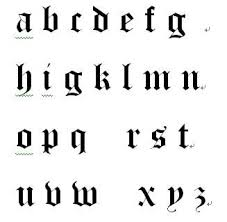
\includegraphics[width=0.7\textwidth]{figures/abc.jpeg} %插入图片,[]中设置图片大小,{}中是图片文件名
\caption{Main name 2} %最终文档中希望显示的图片标题
\label{Fig.main2} %用于文内引用的标签
\end{figure}


\section{多图横排+默认编号}

Figure \ref{Fig.main} has two sub figures, 
fig.\ref{Fig.sub.1} is the travel demand of driving auto, 
and fig. \ref{Fig.sub.2} is the travel demand of park-and-ride.

\begin{figure}[H]
\centering  %图片全局居中
\subfigure[name1]{
\label{Fig.sub.1}
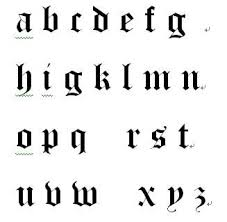
\includegraphics[width=0.45\textwidth]{figures/abc.jpeg}}
\subfigure[name2]{
\label{Fig.sub.2}
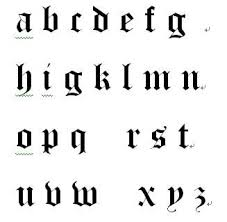
\includegraphics[width=0.45\textwidth]{figures/abc.jpeg}}
\caption{Main name}
\label{Fig.main}
\end{figure}


\section{多图横排+自定义编号}

%注意:此段中在引用中增加了主图编号的引用
Figure \ref{Fig.main} has two sub-figures, 
fig. \ref{Fig.main}\ref{Fig.sub.1} is the travel demand of driving auto, 
and fig. \ref{Fig.main}\ref{Fig.sub.2} is the travel demand of park-and-ride.

%以下code与上一小结的无变化
\begin{figure}[H]
\centering  %图片全局居中
\subfigure[name1]{
\label{Fig.sub.1}
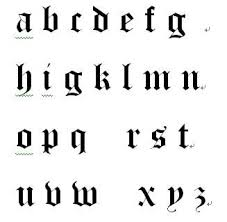
\includegraphics[width=0.45\textwidth]{figures/abc.jpeg}}
\subfigure[name2]{
\label{Fig.sub.2}
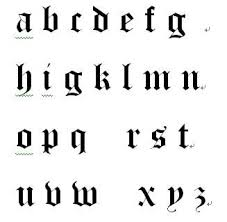
\includegraphics[width=0.45\textwidth]{figures/abc.jpeg}}
\caption{Main name}
\label{Fig.main}
\end{figure}

\section{多图并排显示(非子图模式)}
\subsection{1}
\begin{figure}[H]
\centering %图片全局居中
%并排几个图,就要写几个minipage

\begin{minipage}[b]{0.45\textwidth} %所有minipage宽度之和要小于1,否则会自动变成竖排
\centering %图片局部居中
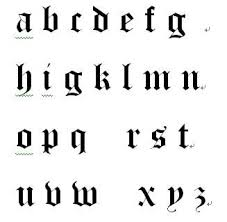
\includegraphics[width=0.8\textwidth]{figures/abc.jpeg} %此时的图片宽度比例是相对于这个minipage的,不是全局
\caption{name 1}
\label{Fig.1}
\end{minipage}
\begin{minipage}[b]{0.45\textwidth} %所有minipage宽度之和要小于1,否则会自动变成竖排
\centering %图片局部居中
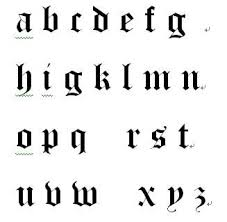
\includegraphics[width=0.8\textwidth]{figures/abc.jpeg}%此时的图片宽度比例是相对于这个minipage的,不是全局
\caption{name 2}
\label{Fig.2}
\end{minipage}

\end{figure}

\subsection{2}
\begin{figure}[H]
\centering %图片全局居中
%并排几个图,就要写几个minipage

\begin{minipage}[b]{0.45\textwidth} %所有minipage宽度之和要小于1,否则会自动变成竖排
\centering %图片局部居中
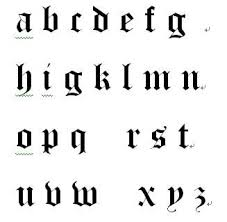
\includegraphics[width=0.8\textwidth]{figures/abc.jpeg} %此时的图片宽度比例是相对于这个minipage的,不是全局
\caption{name 1}
\label{Fig.1}
\end{minipage}

\begin{minipage}[b]{0.45\textwidth} %所有minipage宽度之和要小于1,否则会自动变成竖排
\centering %图片局部居中
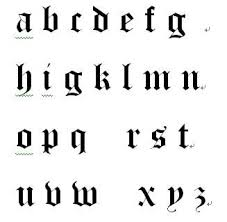
\includegraphics[width=0.8\textwidth]{figures/abc.jpeg}%此时的图片宽度比例是相对于这个minipage的,不是全局
\caption{name 2}
\label{Fig.2}
\end{minipage}

\end{figure}

\subsection{3}
\begin{figure}[H]
    \centering
    \subfigure[子图1]{
    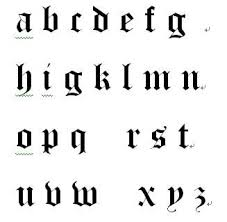
\includegraphics[width=0.2\textwidth]{figures/abc.jpeg}}
    \label{fig:flower}
    \subfigure[子图1]{
    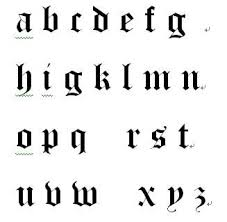
\includegraphics[width=0.2\textwidth]{figures/abc.jpeg}
    \label{fig:car}}
    \subfigure[子图1]{
    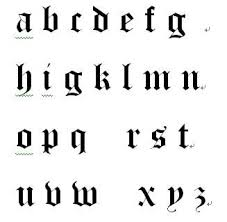
\includegraphics[width=0.2\textwidth]{figures/abc.jpeg}
    \label{fig:ca}}
    \subfigure[子图1]{
    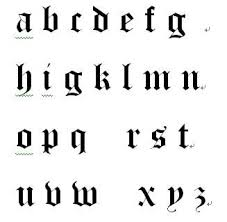
\includegraphics[width=0.2\textwidth]{figures/abc.jpeg}
    \label{fig:cr}}
    \caption{并排图}
\end{figure}
  


    

\end{document}


